% Created 2024-07-28 dom 20:58
% Intended LaTeX compiler: pdflatex
\documentclass[presentation]{beamer}
\usepackage[utf8]{inputenc}
\usepackage[T1]{fontenc}
\usepackage{graphicx}
\usepackage{grffile}
\usepackage{longtable}
\usepackage{wrapfig}
\usepackage{rotating}
\usepackage[normalem]{ulem}
\usepackage{amsmath}
\usepackage{textcomp}
\usepackage{amssymb}
\usepackage{capt-of}
\usepackage{hyperref}
\usetheme{default}
\usecolortheme{}
\usefonttheme{}
\useinnertheme{}
\useoutertheme{}
\author{Enrique Perez S}
\date{<2024-07-2>}
\title{Evidencia Curso Ensamblaje Computadores}

\hypersetup{
 pdfauthor={Enrique Perez S},
 pdftitle={Evidencia Curso Ensamblaje Computadores},
 pdfkeywords={},
 pdfsubject={},
 pdfcreator={Emacs 27.1 (Org mode 9.3)}, 
 pdflang={Spanish}}
\begin{document}

\maketitle
\begin{frame}{Outline}
\tableofcontents
\end{frame}


\section{Conceptos Básicos de Hardware de Computadora}
\label{sec:org5f70ec6}
\begin{frame}[label={sec:orga55e1a3}]{Capturas de pantalla 1}
Captura de pantalla 1
\begin{center}
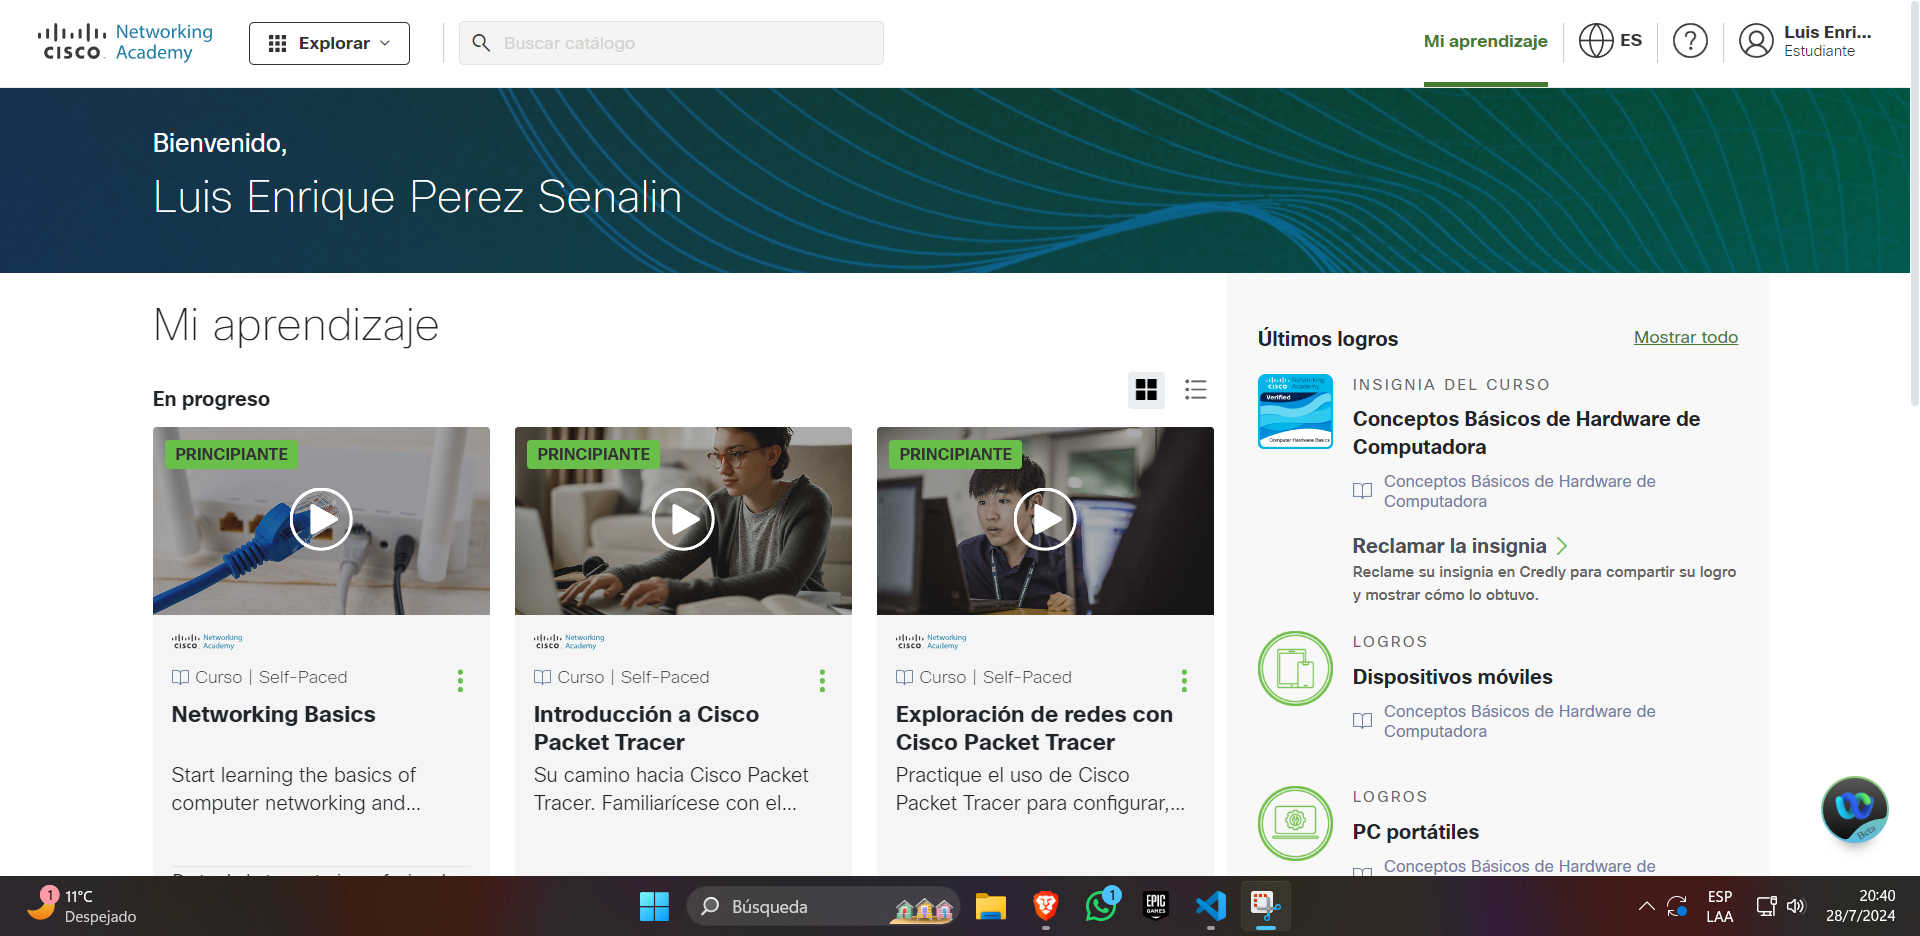
\includegraphics[width=.9\linewidth]{./dashboard.png}
\end{center}
\end{frame}
\begin{frame}[label={sec:orgbcb7a69}]{Capturas de pantalla 2}
Captura de pantalla 2
\begin{center}
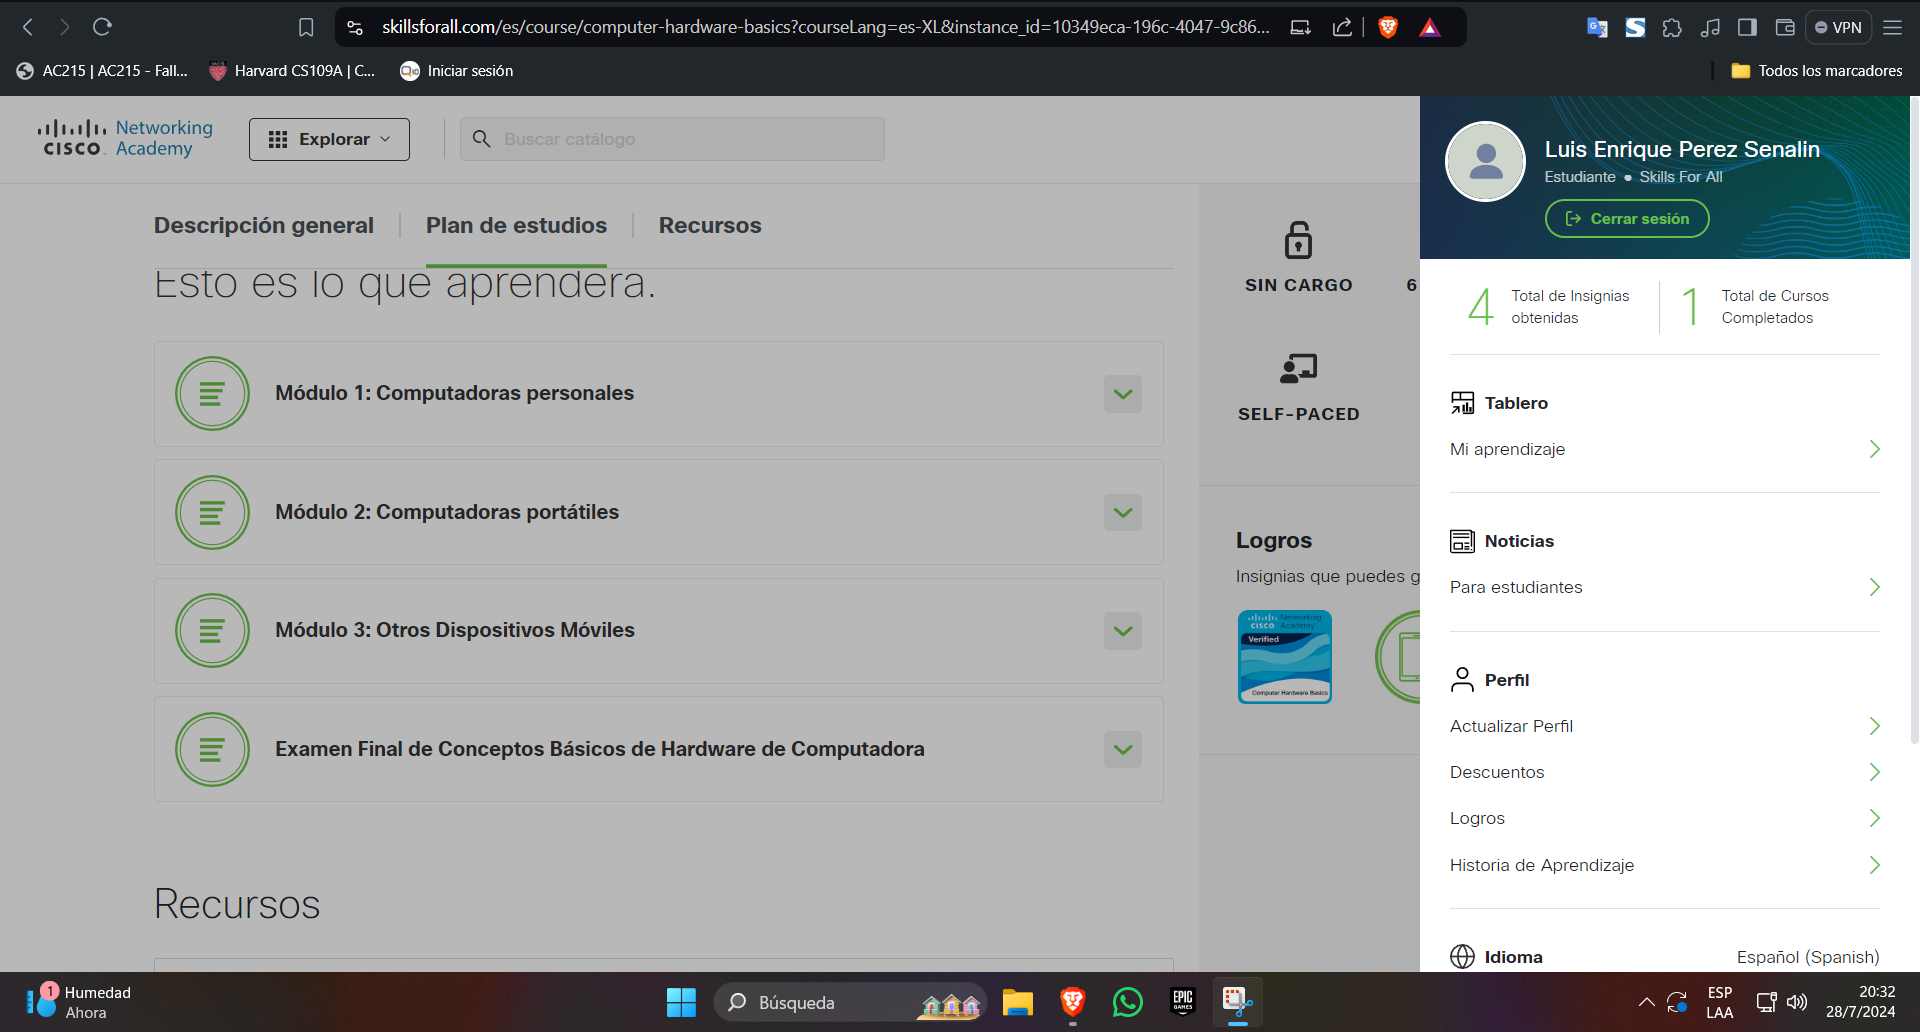
\includegraphics[width=.9\linewidth]{./todas_secciones.png}
\end{center}
\end{frame}

\section{Comentarios}
\label{sec:orgbd085da}
\begin{frame}[label={sec:org31b0eda}]{Sección de Comentarios}
El curso es bastante bueno, explicame de forma completa muchas secciones $$\n$$
Tiene algunos problemas en las preguntas, pero son pocos. $$\n$$
El curso debe actualizar el hardware que se utiliza porque actualmente han habido muchos cambios, pero en su mayoría sigue siendo útil

La mayoría de los conocimientos ya los he tendio así que solo unos cuantos temas nuevos he visto.
\end{frame}
\end{document}
